\IEEEraisesectionheading{\label{sec:introduction}}
\section{INTRODUCTION}
\IEEEPARstart{R}{estoring} a power cyber-physical system (PCPS) after a disruptive event requires a feasible electrical configuration and a usable cyber path for carrying out the corresponding actions. Controller status, command reachability, measurement trust, protection state, and recent recovery outcomes all enter that decision. Electrical feasibility alone does not make a switching action executable: the controller and command path must also be available. A stale measurement can support the wrong reconfiguration, and a manipulated outcome record can later be reused as evidence for another action. We treat these runtime dependencies as part of the recovery state whose integrity must be protected. Fig.~\ref{fig-scenario} shows the cross-layer setting.

\begin{figure*}[t]
\centering
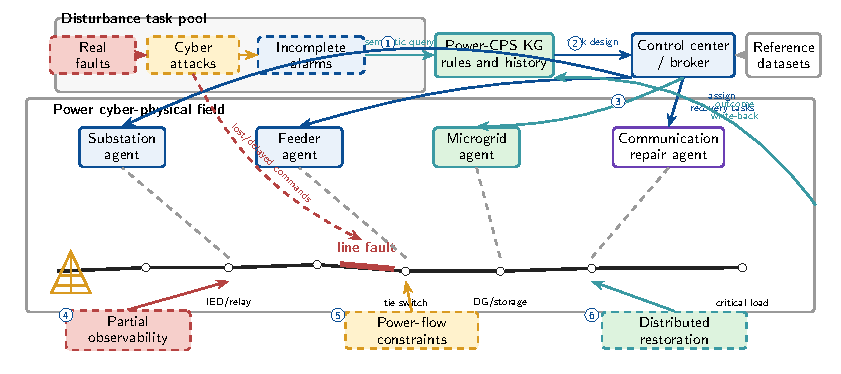
\includegraphics[width=\textwidth]{figures/power_cps_scenario.pdf}
\caption{Illustrative recovery setting in a power cyber-physical system. Physical faults, impaired communication, and incomplete or corrupted observations jointly determine which restoration actions can be trusted and executed.}
\label{fig-scenario}
\end{figure*}

Resilient CPS research has studied cross-layer dependencies among cyber, communication, control, and physical components \cite{zhu2020cross,liao2025surveyresilient}. Existing methods include game-theoretic resilient control, secure or resilient model predictive control, and observer/event-triggered designs for denial-of-service, false-data-injection, and hybrid attacks \cite{game2026hybrid,resilientmpc2025dos,stochastic2025tube,sampled2025observer}. Power-system restoration models have also incorporated communication impairment and cyber-physical operating constraints into reconfiguration and service recovery \cite{zhou2025faultresilient}. In these formulations, runtime inputs usually appear as measurements, estimated states, attack estimates, communication states, or predefined constraints. Recovery studies also make explicit assumptions about diagnosis, attack history, and the recovery module \cite{lu2024recovery}. What remains less explicit is the integrity of a reusable knowledge state assembled from these inputs and later used to authorize recovery actions.

Knowledge graphs (KGs) are useful for representing such dependencies as typed, queryable relations. General KG work covers heterogeneous entities and relations, context, validation, inference, and graph learning \cite{hogan2021knowledgegraphs,reinanda2020knowledge}. CPS studies have used KGs for time-continuous behavior, weighted information dependencies, cross-domain threat modeling, and control reconfiguration \cite{liu2025timecontinuous,wang2025weightedkg,wu2026multidimensional,knowledge2025dynamic}. Incremental causal graphs and KG-assisted verification have also been explored for online attack detection \cite{incremental2026causal,hybridtcdf2026}. These capabilities do not by themselves determine whether the evidence that created a runtime assertion is trustworthy. Three reports can be syntactically distinct yet share one compromised gateway; a valid old report can be replayed after the operating condition has changed. Both cases can alter a graph state without violating its schema.

We call this attack surface \emph{recovery knowledge poisoning}. The path of interest is
\begin{align}
\label{eq-intro-propagation}
&\text{adversarial evidence}\rightarrow\text{recovery knowledge}\nonumber\\
&\qquad\rightarrow\text{action authority}\rightarrow\text{online policy}.
\end{align}
Consider a fabricated controller-availability report. If it is accepted as ordinary recovery knowledge, a remote switching action can pass a semantic prerequisite even though the controller is unavailable. The resulting transition may then enter replay and influence later policy updates after the original report has expired. This is the point at which anomaly detection, a physical safety check, and robust policy optimization solve different problems: none of them alone controls the whole evidence-to-knowledge-to-learning path.

KG-FedMARL addresses that path at three places. Runtime assertions are maintained as temporal beliefs with source identity and provenance. Evidence is calibrated, aged, and grouped by provenance so that one correlated source group has bounded influence. Recovery actions use these beliefs only for evidence-dependent prerequisites; invariant engineering constraints remain the responsibility of an authoritative physical verifier over a conservative state set. A learned surrogate may rank candidates, but it cannot approve field execution.

Online learning uses a separate, slower trust boundary. Each transition is tied to the belief, policy, and verifier versions present at execution. New transitions remain in quarantine until their supporting beliefs, provenance coverage, evidence completeness, and outcomes meet the promotion criteria. Stable and candidate policies are kept separate, and candidate promotion is restricted by a trust-dependent KL radius and shadow evaluation through the same recovery gate. Federated training, heterogeneous action heads, and graph encoders can be used in an implementation, but they have no authority to bypass the local gate or verifier.

We formulate restoration as a constrained decentralized partially observable Markov decision process with four security quantities: belief distortion under bounded evidence compromise, semantic false authorization, correction time after trustworthy evidence resumes, and deviation of the deployed policy. Section~VI derives sufficient bounds for these quantities from the provenance budgets, forgetting factor, calibration error, and policy-promotion constraints. The guarantees are limited to the trust boundary stated in Section~III; they are not a convergence proof for a nonlinear MARL optimizer.

The paper makes three contributions.
\begin{itemize}
\item \emph{Recovery-knowledge threat model.} We define recovery knowledge poisoning for bounded source compromise, fabrication, suppression, replay, delay, and provenance correlation. The model separates protected semantic invariants from runtime assertions inferred from evidence.

\item \emph{Recovery mechanisms with explicit trust boundaries.} KG-FedMARL combines provenance-bounded temporal belief updates, a semantic recovery gate followed by authoritative physical verification, and quarantined online policy adaptation with stable--candidate separation.

\item \emph{Security bounds tied to the recovery pipeline.} We bound belief distortion, semantic false-authorization probability, post-attack correction time, and cumulative deployed-policy drift under the stated assumptions, and evaluate the same quantities in controlled and feeder-level experiments.
\end{itemize}

Section~II reviews related work. Section~III defines the system and threat model. Section~IV gives the restoration formulation and security objectives. Section~V presents KG-FedMARL, Section~VI gives the security analysis, and Section~VII reports the experiments.
